\subsection{Use Case Diagram}
\label{diagram:usecase}
I meccanismi base di individuazione e definizione dei casi d'uso son già stati esplicati nella \hyperref[concept:casi-duso]{sezione dedicatali}. In questa sezione pertanto ci si limiterà a presentare il diagramma dei casi d'uso, tenendo conto della sua notazione grafica e di eventuali meccanismi avanzati legati all'uso degli UC. \\
I diagrammi dei \hyperref[concept:casi-duso]{casi d'uso} (o \textbf{Use Cases Diagram}) sono uno strumento dell'UML utilizzato per rappresentare tutti i casi d'uso presenti nel sistema e gli attori che li attivano. \\
L'obiettivo è mostrare quali sono le funzionalità del sistema, senza entrare nei dettagli implementativi del come vengono ottenute. Ogni \hyperref[concept:casi-duso]{UC} descrive un'interazione significativa tra un attore e il sistema stesso, finalizzata a raggiungere un certo obiettivo. \\
Un diagramma dei casi d'uso è quindi uno dei primi diagrammi da sviluppare in sviluppo ed è composto da:
\begin{itemize}
    \item \textbf{Attori} che rappresentano chi interagisce con il sistema attivando i casi d'uso. Sono rappresentati da uno stickman.
    \item \textbf{Casi d'uso} che rappresentano le funzionalità fornite dal sistema, rappresentati da un ovale.
    \item \textbf{Relazioni} tra attori e casi d'uso (attivazione) e tra casi d'uso stessi (inclusione, estensione, generalizzazione). Rappresentati attraverso delle linee.
    \item \textbf{Dominio} limiti del sistema o componente a cui sono associati determinati casi d'uso. Rappresentati da rettangoli.
\end{itemize}
\begin{figure}[h]
    \centering
    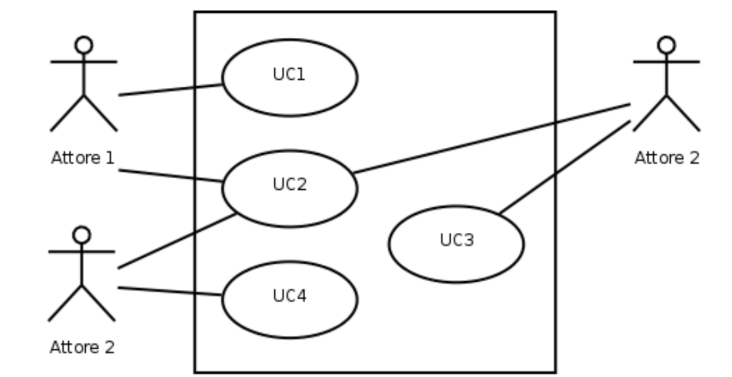
\includegraphics[width=0.80\linewidth]{IDSTEORIA/Immagini/UML/UC_base.png}
    \caption{Rappresentazione base di un diagramma dei casi d'uso.}
    \label{fig:uc_base}
\end{figure}
\subsubsection{Meccanismi avanzati}
UML mette a disposizione alcuni meccanismi avanzati per la rappresentazione degli UC. \\
Nello specifico:
\begin{itemize}
    \item \textbf{Generalizzazione degli attori}, attori con comportamenti o UC attivabili in comune possono essere generalizzati da un unico attore.
    \item \textbf{Generalizzazione tra casi d'uso}, i casi d'uso possono ereditare, aggiungere o ridefinire comportamenti da altri UC.
    \item \textbf{Inclusione $<<$include$>>$}, riutilizzare comportamenti comuni tra casi d'uso.
    \item \textbf{Estensione $<<$extend$>>$}, permette di aggiungere funzionalità opzionali o condizionali.
\end{itemize}
\begin{figure}[h]
    \centering
    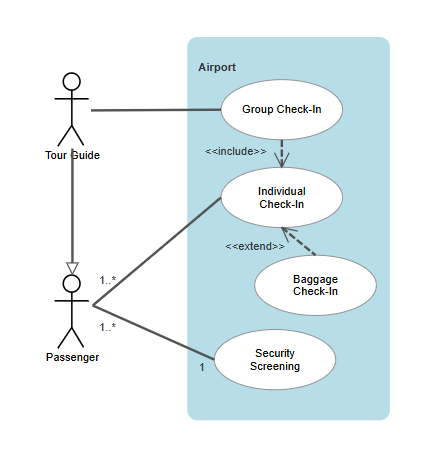
\includegraphics[width=0.7\linewidth]{IDSTEORIA/Immagini/UML/Esempio_UC_Diagram.png}
    \caption{Esempio di Use Cases Diagram che fa uso dei meccanismi avanzati.}
    \label{fig:UC_avanzato}
\end{figure}
Ad esempio, nella Figure \ref{fig:UC_avanzato}, l'attore Tour Guide è una composizione di attori Passenger. L'attore Tour Guide può inoltre attivare un solo caso d'uso: Group Check-in. Quest'ultimo caso d'uso include al suo interno il caso d'uso Individual Check-in, che a sua volta viene esteso da Baggage Check-in. 